\documentclass[UTF8]{article}
\usepackage{graphicx}
\usepackage{subfigure}
\usepackage{amsmath}
\usepackage{makecell}
\usepackage[utf8]{inputenc}
\usepackage[space]{ctex} %中文包
\usepackage{listings} %放代码
\usepackage{xcolor} %代码着色宏包
\usepackage{CJK} %显示中文宏包
\usepackage{float}
\usepackage{makecell}
\usepackage{diagbox}
\usepackage{bm}
\usepackage{ulem} 
\usepackage{amssymb}
\usepackage{soul}
\usepackage{color}
\usepackage{geometry}
\usepackage{fancybox} %花里胡哨的盒子
\usepackage{xhfill} %填充包, 可画分割线 https://www.latexstudio.net/archives/8245
\usepackage{multicol} %多栏包
\usepackage{enumerate} %可以方便地自定义枚举标题
\usepackage{multirow} %表格中多行单元格合并
\usepackage{wasysym} %可以使用wasysym里的一堆奇奇怪怪的符号
\usepackage{mips}

\geometry{left = 2.5cm, right = 2.5cm}

\definecolor{mygreen}{rgb}{0,0.6,0}
\definecolor{mygray}{rgb}{0.5,0.5,0.5}
\definecolor{mymauve}{rgb}{0.58,0,0.82}
\lstset{ %
	language=[mips]Assembler,       % the language of the code
	basicstyle=\footnotesize,       % the size of the fonts that are used for the code
	numbers=left,                   % where to put the line-numbers
	numberstyle=\tiny\color{gray},  % the style that is used for the line-numbers
	stepnumber=1,                   % the step between two line-numbers. If it's 1, each line
	% will be numbered
	numbersep=5pt,                  % how far the line-numbers are from the code
	backgroundcolor=\color{white},  % choose the background color. You must add \usepackage{color}
	showspaces=false,               % show spaces adding particular underscores
	showstringspaces=false,         % underline spaces within strings
	showtabs=false,                 % show tabs within strings adding particular underscores
	frame=single,                   % adds a frame around the code
	rulecolor=\color{black},        % if not set, the frame-color may be changed on line-breaks within not-black text (e.g. commens (green here))
	tabsize=4,                      % sets default tabsize to 2 spaces
	captionpos=b,                   % sets the caption-position to bottom
	breaklines=true,                % sets automatic line breaking
	breakatwhitespace=false,        % sets if automatic breaks should only happen at whitespace
	title=\lstname,                 % show the filename of files included with \lstinputlisting;
	% also try caption instead of title
	keywordstyle=\color{blue},          % keyword style
	commentstyle=\color{green},       % comment style
	stringstyle=\color{mauve},         % string literal style
	escapeinside={\%*}{*)},            % if you want to add a comment within your code
	morekeywords={*,...}               % if you want to add more keywords to the set
}

%\sum\nolimits_{j=1}^{M}   上下标位于求和符号的水平右端,
%\sum\limits_{j=1}^{M}   上下标位于求和符号的上下处,
%\sum_{j=1}^{M}  对上下标位置没有设定,会随公式所处环境自动调整。

%%%%%%%%%%%%%画图包%%%%%%%%%%%%%
\usepackage{tikz}
%%%%%%%%%%%%%画图背景包%%%%%%%%%%%%%
\usetikzlibrary{backgrounds}

%%%%%%%%%%%%%在tikz中画一个顶点%%%%%%%%%%%%%
%%%%%%%%%%%%%#1:node名称%%%%%%%%%%%%%
%%%%%%%%%%%%%#2:位置%%%%%%%%%%%%%
%%%%%%%%%%%%%#3:标签%%%%%%%%%%%%%
\newcommand{\newVertex}[3]{\node[circle, draw=black, line width=1pt, scale=0.8] (#1) at #2{#3}}
%%%%%%%%%%%%%在tikz中画一条边%%%%%%%%%%%%%
\newcommand{\newEdge}[2]{\draw [black,very thick](#1)--(#2)}
%%%%%%%%%%%%%在tikz中放一个标签%%%%%%%%%%%%%
%%%%%%%%%%%%%#1:名称%%%%%%%%%%%%%
%%%%%%%%%%%%%#2:位置%%%%%%%%%%%%%
%%%%%%%%%%%%%#3:标签内容%%%%%%%%%%%%%
\newcommand{\newLabel}[3]{\node[line width=1pt] (#1) at #2{#3}}

%%%%%%%%%%%%%强制跳过一行%%%%%%%%%%%%%
\newcommand{\jumpLine} {\hspace*{\fill} \par}
%%%%%%%%%%%%%关键点指令,可用itemise替代%%%%%%%%%%%%%
\newcommand{\average}[1]{\left\langle #1\right\rangle }
%%%%%%%%%%%%%表格内嵌套表格%%%%%%%%%%%%%

\newcommand{\keypoint}[2]{$\bullet$\textbf{#1}\quad#2\par}
%%%%%%%%%%%%%<T>平均值表示%%%%%%%%%%%%%
\newcommand{\tabincell}[2]{\begin{tabular}{@{}#1@{}}#2\end{tabular}}%放在导言区
%%%%%%%%%%%%%大黑点item头%%%%%%%%%%%%%
\newcommand{\itemblt}{\item[$\bullet$]}
%%%%%%%%%%%%%大圈item头%%%%%%%%%%%%%
\newcommand{\itemc}{\item[$\circ$]}
%%%%%%%%%%%%%大星星item头%%%%%%%%%%%%%
\newcommand{\itembs}{\item[$\bigstar$]}
%%%%%%%%%%%%%右▷item头%%%%%%%%%%%%%
\newcommand{\itemrhd}{\item[$\rhd$]}
%%%%%%%%%%%%%定义为%%%%%%%%%%%%%
\newcommand{\defas}{=_{df}}
%%%%%%%%%%%%%蕴含%%%%%%%%%%%%%
\newcommand{\imp}{\rightarrow}

%%%%%%%%%%%%%双线分割线%%%%%%%%%%%%%
\newcommand*{\doublerule}{\hrule width \hsize height 1pt \kern 0.5mm \hrule width \hsize height 2pt}
%%%%%%%%%%%%%双线中间可加东西的分割线%%%%%%%%%%%%%
\newcommand\doublerulefill{\leavevmode\leaders\vbox{\hrule width .1pt\kern1pt\hrule}\hfill\kern0pt }
%%%%%%%%%%%%%左大括号%%%%%%%%%%%%%
\newcommand{\leftbig}[1]{\left\{\begin{array}{l}#1\end{array}\right.}
%%%%%%%%%%%%%矩阵%%%%%%%%%%%%%
\newcommand{\mat}[2]{\left[\begin{array}{#1}#2\end{array}\right]}
%%%%%%%%%%%%%可换行圆角文本框%%%%%%%%%%%%%

\newcommand{\ovalboxn}[1]{\ovalbox{\tabincell{l}{#1}}}
%%%%%%%%%%%%%设置section的counter, 使从0开始%%%%%%%%%%%%%
\setcounter{section}{0}







\title{计算机组成原理MIPS实验}
\date{}
%\author{王章瀚 PB18111697}


\begin{document}

%%%%%%%%%%%%%科大报告封面%%%%%%%%%%%%%
\maketitle
\begin{figure}[H]
	\centering
	
\includegraphics[width=2.5in]{xiaohui.png}\vspace{0.5cm}\\
	\large{
		实验题目: MIPSS冒泡排序\\
		学生姓名:王章瀚\\
		学生学号:PB18111697\\
		完成日期:\today\\
	}\vspace{2cm}
	
	\large{计算机实验教学中心制\\2019年09月\\}
	\thispagestyle{empty}
	\clearpage  % 清除当页页码
\end{figure}
\newpage

\section{题目要求}
\begin{enumerate}
	\item 基于MIPS汇编,设计一个冒泡排序程序,并用Debug工具调试执行。
	\item 测量冒泡排序程序的执行时间。
	\item 提交实验报告,并在报告后附上源码。
	\item 不强制提交,但写了会有额外加分,具体加分待定。
\end{enumerate}

\section{代码结构分析}
\subsection{函数说明}
\subsubsection{main}
用以调用随机数组生成函数和冒泡排序函数,并在此计时,最终输出时间。
\subsubsection{array\_generate}
传入参数为: 
\begin{itemize}
	\item \$a0: 数组起始地址
	\item \$a1: 数组大小
\end{itemize}
最后会在数组起始地址开始,生成数组大小的个数的随机数,这里随机数小于等于10000。
\subsubsection{bubble\_sort}
传入参数为: 
\begin{itemize}
	\item \$a0: 数组起始地址
	\item \$a1: 数组大小
\end{itemize}
这个函数实现了对数组起始地址开始数组大小个数的元素的冒泡排序(此处是从小到大)。冒泡排序算法比较出名,通过两个循环,每次把最大的数移到最末位,这里就不再赘述其原理了。

\section{代码运行结果}
这里放一张代码运行结果的截图,以证明确实完成了排序。
\begin{figure}[H]
	\centering
	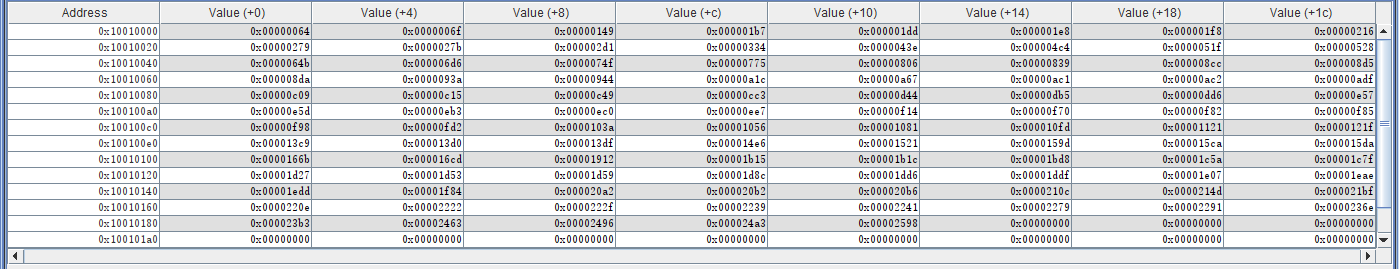
\includegraphics[scale=0.36]{sort_100.png}
\end{figure}\par
可以看到从0x10010004开始的100个数都按从小到大的顺序排好了。


\section{代码时间测量}
\subsection{测量结果}
时间测量部分以数组大小为变量测量了多组数据,如下表所示:
\begin{figure}[H]
	\centering
	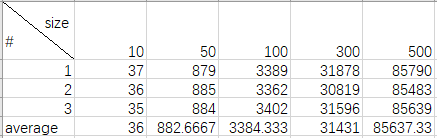
\includegraphics[scale=0.8]{test_result.png}
\end{figure}\par

然后用Python程序对数据进行了二次函数拟合,结果如下图
\begin{figure}[H]
	\centering
	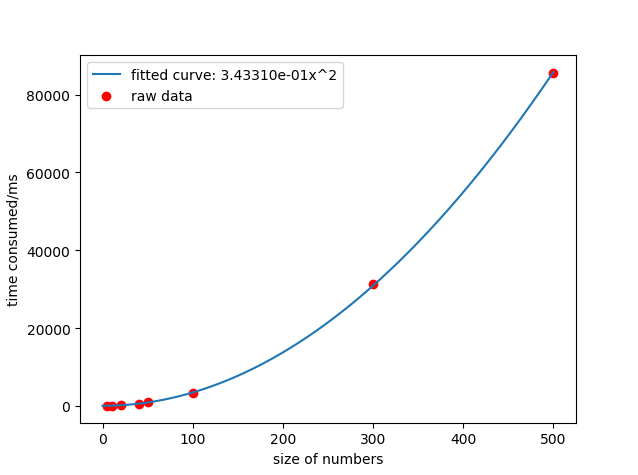
\includegraphics[scale=0.6]{test_diagram.png}
\end{figure}\par
\subsection{结果说明}
可以看到,冒泡排序的时间随数组大小成二次函数的关系,这是符合冒泡排序的$o(n^2)$的时间复杂度的。

\section{总结}
本次实验用MIPS汇编实现了冒泡排序,并验证了冒泡排序$o(n^2)$的时间复杂度。

\section{附代码}
\lstinputlisting{bubble_sort.asm}


\end{document}




